%! TEX root = ../thesis.tex

\chapter{The Pierre Auger Observatory}
\label{chap:auger-observatory}

Located on the argentinian high-plains of Pampa Amarilla, the Pierre Auger observatory is a hybrid detector designed to detect and study cosmic 
rays of the highest energies. With an effective area of \SI{3000}{\kilo\meter\squared} it is by far the largest experiment of its kind 
\cite{DesignReport}.

This chapter offers a brief look into the measurement principle and setup of the observatory. The  surface detector (SD) is described in 
\autoref{sec:surface-detector} and critical in understanding the analysis presented in \autoref{chap:station-triggers}. For a more complete 
overview on the experiment, information regarding the fluoresence detector can be found in \autoref{sec:fluoresence-detector}. Notes on the event
reconstruction are found in \autoref{sec:event-reconstruction}. If not explicitly stated otherwise, information is adpoted from the Pierre Auger 
observatory design report \cite{DesignReport}.

\begin{figure}
	\centering
	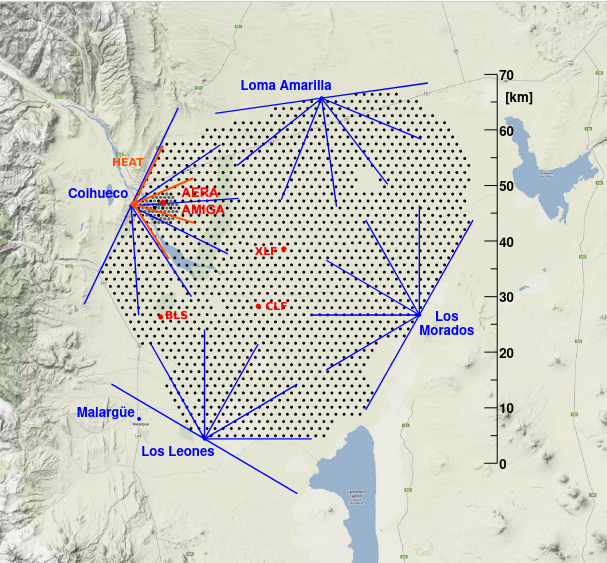
\includegraphics[width=0.9\textwidth]{plots/auger_array.png}
	\caption{Overview of the Pierre Auger observatory. The four different FD sites (respective FOV shown with blue lines) sit at the edge of
	the detector area and monitor the night sky above the SD array consisting of 1600 water tanks (black dots). Two laser facilities, the 
	e\textbf{X}treme (XLF) and \textbf{C}entral \textbf{L}aser \textbf{F}acility (CLF) are located in the middle of the array to measure 
	atmospheric properties. A denser spacing of stations near Coihueco is equipped with additional electronics such as e.g. radio antennas 
	(AERA) and muon detectors (AMIGA).}
	\label{fig:auger-array}
\end{figure}

\section{Fluoresence Detector (FD)}
\label{sec:fluoresence-detector}

The fluoresence detector consists of a total of 27 fluoresence telescopes at 4 different sites (compare \autoref{fig:auger-array}). Each telescope
monitors a \SI{30}{\degree} x \SI{30}{\degree} window of the night sky. This results in an effective FOV of roughly \SI{180}{\degree} x 
\SI{30}{\degree} per FD station, with an exception of Coihueco, where three additional telescopes (\textbf{H}igh \textbf{E}levation \textbf{A}uger
\textbf{T}elescope) are installed to enable monitoring of higher zenith angles ($\SI{30}{\degree}\leq\theta\leq\SI{60}{\degree}$) to increase
sensitivity for showers of lower energies (compare \autoref{chap:physical-background}).

The individual telescopes consists of a \SI{3.6}{\meter} by \SI{3.6}{\meter}, curved mirror, which reflect light onto 440 photomultipliers (PMTs)
that make up the pixels of the photo sensor. Since the setup needs to be extremely sensitive to UV light in order to see traces of air showers, 
its operation is limited to the argentinian nautical (? \TODO) night.

\section{Surface Detector (SD)}
\label{sec:surface-detector}

the surface detector consists of a multitude of individually operating stations. Each station is made up of a \SI{12000}{\litre} tank filled with 
highly purified water and equipped with three PMTs that detect Cherenkov light. Gathered data  

\section{Trigger Procedure and Event Reconstruction}
\label{sec:event-reconstruction}


